\documentclass[letterpaper,11pt,oneside,reqno]{article}

%%%%%%%%%%%%%%%%%%%%%%%%%%%%%%%%%%%%%%%%%%%%%%%%%%%%%%%%%%%%

\usepackage[pdftex,backref=page,colorlinks=true,linkcolor=blue,citecolor=red]{hyperref}
\usepackage[alphabetic,nobysame]{amsrefs}

%%%%%%%%%%%%%%%%%%%%%%%%%%%%%%%%%%%%%%%%%%%%%%%%%%%%%%%%%%%%
%main packages
\usepackage{amsmath,amssymb,amsthm,amsfonts,mathtools}
\usepackage{graphicx,color}
\usepackage{upgreek}
\usepackage[mathscr]{euscript}

%equations
\allowdisplaybreaks
\numberwithin{equation}{section}

%tikz
\usepackage{tikz}
\usetikzlibrary{shapes,arrows,positioning,decorations.markings}

%conveniences
\usepackage{array}
\usepackage{adjustbox}
\usepackage{cleveref}
\usepackage{enumerate}
\usepackage{datetime}

%paper geometry
\usepackage[DIV=12]{typearea}

%%%%%%%%%%%%%%%%%%%%%%%%%%%%%%%%%%%%%%%%%%%%%%%%%%%%%%%%%%%%
%draft-specific
\synctex=1
% \usepackage{refcheck,comment}

%%%%%%%%%%%%%%%%%%%%%%%%%%%%%%%%%%%%%%%%%%%%%%%%%%%%%%%%%%%%
%this paper specific
\newcommand{\ssp}{\hspace{1pt}}

%%%%%%%%%%%%%%%%%%%%%%%%%%%%%%%%%%%%%%%%%%%%%%%%%%%%%%%%%%%%
\newtheorem{proposition}{Proposition}[section]
\newtheorem{lemma}[proposition]{Lemma}
\newtheorem{corollary}[proposition]{Corollary}
\newtheorem{theorem}[proposition]{Theorem}
%%%%%%%%%%%%%%%%%%%%%%%%%%%%%%%%%%%%%%%%%%%%%%%%%%%%%%%%%%%%
\theoremstyle{definition}
\newtheorem{definition}[proposition]{Definition}
\newtheorem{remark}[proposition]{Remark}
%%%%%%%%%%%%%%%%%%%%%%%%%%%%%%%%%%%%%%%%%%%%%%%%%%%%%%%%%%%%

\begin{document}
\title{Lectures on Random Matrices
(Spring 2025)
\\Lecture 12: Random Growth Models}


\date{Wednesday, April 2, 2025\footnote{\href{https://lpetrov.cc/rmt25/}{\texttt{Course webpage}}
$\bullet$ \href{https://lpetrov.cc/simulations/model/random-matrices/}{\texttt{Live simulations}}
$\bullet$ \href{https://lpetrov.cc/rmt25/rmt25-notes/rmt2025-l12.tex}{\texttt{TeX Source}}
$\bullet$
Updated at \currenttime, \today}}



\author{Leonid Petrov}


\maketitle
\tableofcontents


\section{Recap}

In our last lecture, we explored the asymptotics of Dyson Brownian Motion with an outlier. We specifically focused on the phase transition that occurs when a rank-1 perturbation is applied to a random matrix ensemble.

\subsection{Dyson Brownian Motion with Determinantal Structure}

We established that for $\beta=2$, the eigenvalues of the time-evolved process form a determinantal point process. The transition probability from an initial configuration $\mathbf{a} = (a_1 \geq \cdots \geq a_N)$ to a configuration $\mathbf{x} = (x_1 \geq \cdots \geq x_N)$ at time $t$ is given by:
\begin{equation*}
P(\lambda(t) = \mathbf{x} \mid \lambda(0) = \mathbf{a}) = N! \Big(\frac{1}{\sqrt{2\pi t}}\Big)^N \prod_{1\leq i<j\leq N}\frac{x_i - x_j}{a_i - a_j} \det\Big[\exp\Big(-\frac{(x_i - a_j)^2}{2t}\Big)\Big]_{i,j=1}^N
\end{equation*}

This determinantal structure enabled us to derive the correlation kernel:
\begin{equation}\label{eq:correlation-kernel}
K_t(x,y) = \frac{1}{(2\pi)^2 t} \int\int \exp\Big(\frac{w^2 - 2yw}{2t}\Big) \bigg/ \exp\Big(\frac{z^2 - 2xz}{2t}\Big) \prod_{i=1}^n \frac{w-a_i}{z-a_i} \frac{dw\,dz}{w-z}
\end{equation}
where the contours of integration are specified to maintain analytical properties.

\subsection{The BBP Phase Transition}

The central focus was the Baik-Ben Arous-Péché (BBP) phase transition that occurs with finite-rank perturbations of GUE matrices. For the rank-1 case, we analyzed:
\begin{equation*}
A + \sqrt{t}G, \quad \text{where } A = \text{diag}(a\sqrt{n},0,\ldots,0)
\end{equation*}

Through asymptotic analysis using steepest descent methods, we identified three distinct regimes:

\begin{enumerate}
\item \textbf{Airy regime} ($a < 1$): The largest eigenvalue follows the Tracy-Widom GUE distribution, just as in the unperturbed case. The spike is too weak to escape the bulk.

\item \textbf{Critical regime} ($a = 1$): A transitional behavior occurs when $a = 1 + An^{-1/3}$, leading to a deformed Airy kernel:
\begin{equation*}
\tilde{K}_{\text{Airy}}(\xi,\eta) = \frac{1}{(2\pi i)^2}\iint \frac{\exp\left\{\frac{W^3}{3}-\xi W-\frac{Z^3}{3}+\eta Z\right\}}{W-Z} \frac{W-A}{Z-A} dW\,dZ
\end{equation*}

\item \textbf{Gaussian regime} ($a > 1$): The largest eigenvalue separates from the bulk, becoming an "outlier" centered at $a + 1/a$. Its fluctuations follow a Gaussian distribution rather than the Tracy-Widom law.
\end{enumerate}


\subsection{Remark: Corners process with outliers}

One can also perturb the corners process structure, and get
correlation kernels similar to \eqref{eq:correlation-kernel}
which we had for the Dyson Brownian Motion.
The perturbed corners process is
considered in \cite{Ferrari2014PerturbedGUE},
see also the earlier work \cite{Metcalfe2011GT}
for the corners process of $UDU^\dagger$, where $D$ is arbitrary and
$U$ is Haar-distributed. Both the kernels
for the Dyson Brownian Motion and the corners process
with outliers can be obtained from the formula of
\cite{Metcalfe2011GT}.
See \Cref{fig:outlier-evolution} for an illustration of the corners process with an outlier
in two cases, when the basis for the outlier is rotated or not
(the rotation does not affect the top level eigenvalue distribution,
but has a significant effect on the whole corners process).




\begin{figure}[]
	\centering
	\begin{tabular}{cc}
		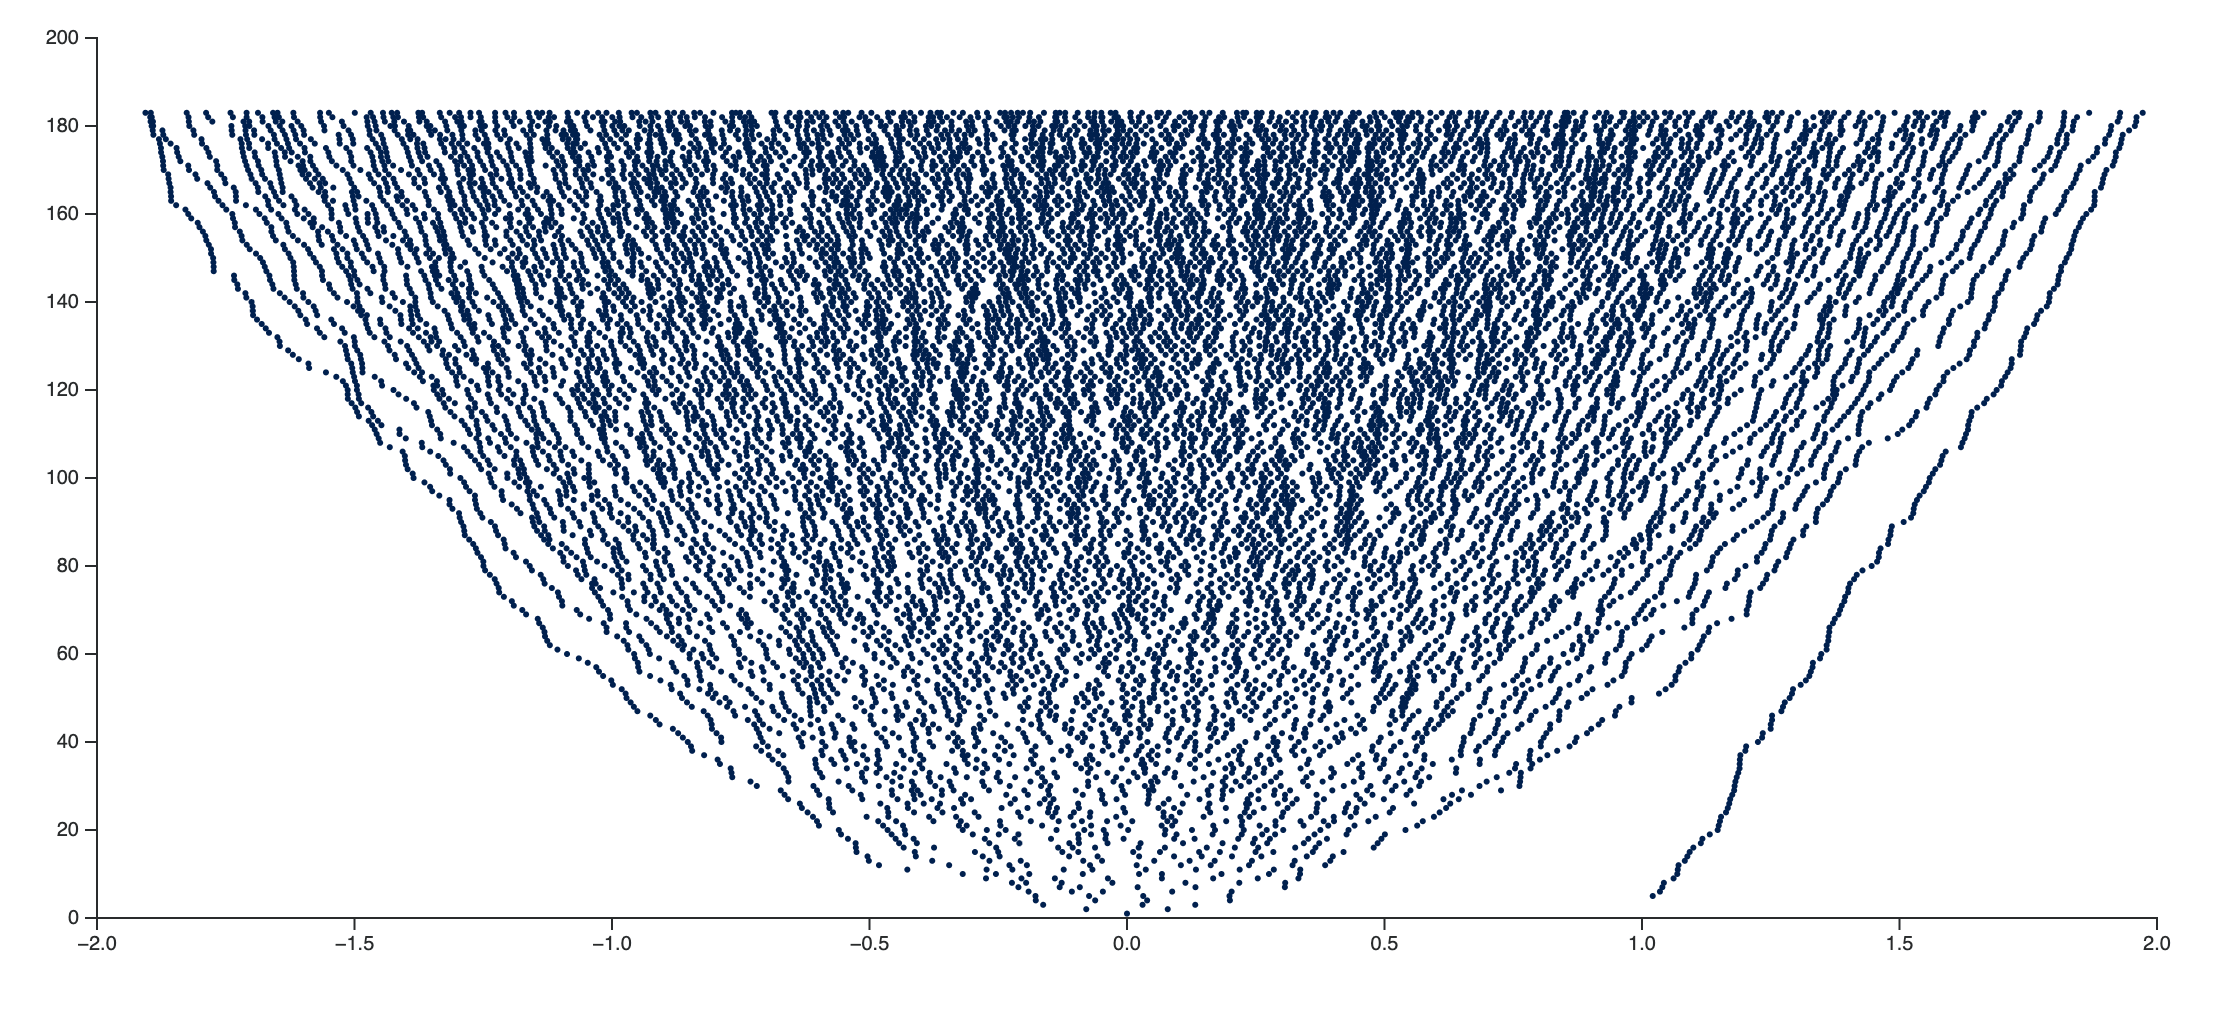
\includegraphics[width=0.45\textwidth]{pictures/outlier.png} &
		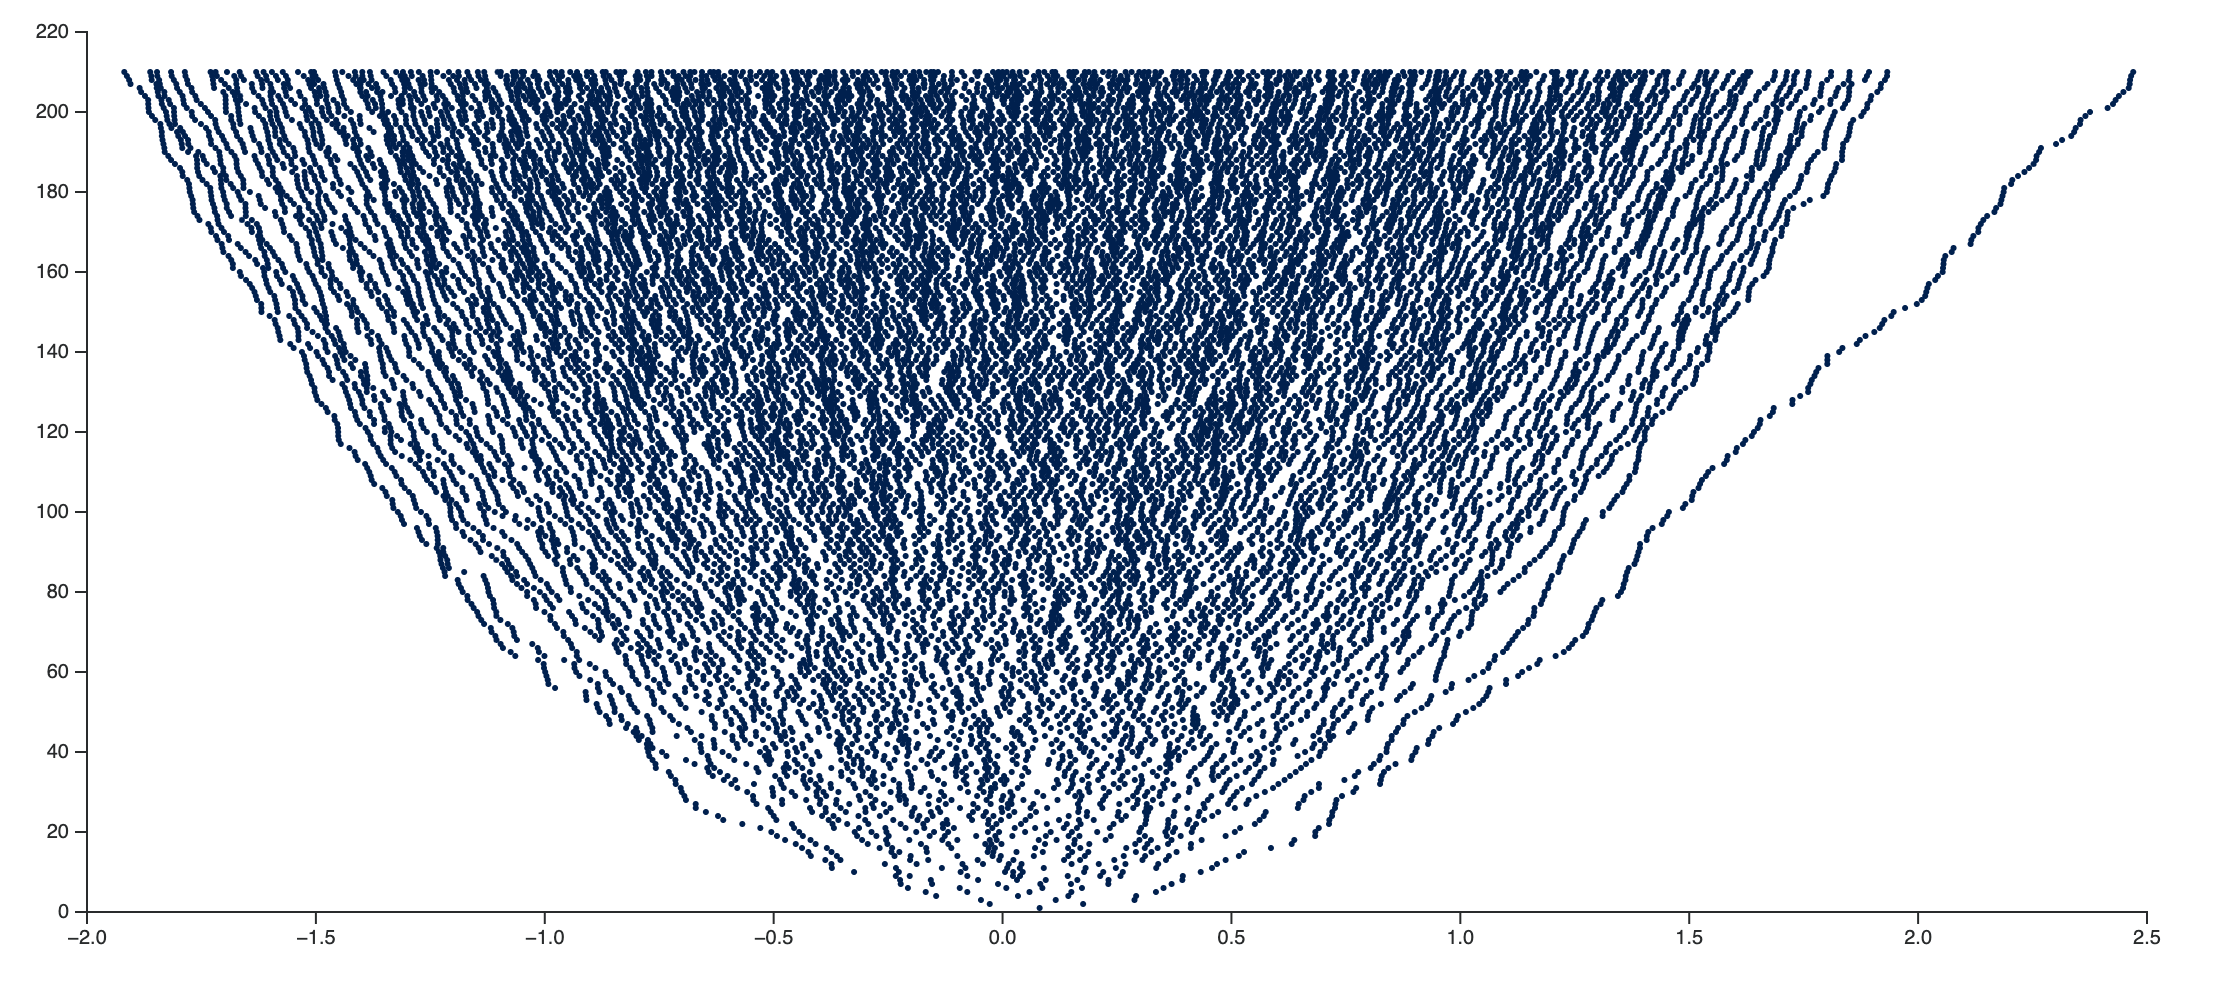
\includegraphics[width=0.45\textwidth]{pictures/rotated_outlier.png}
	\end{tabular}
	\caption{Two versions of the corners process with an outlier.
	Left: Corners process of $G+D$, where $D$ is a rank-1 critical perturbation with eigenvalue
	$1$. Right: Corners process of $G+UDU^\dagger$, where
	$U\in U(n)$ is a Haar-distributed unitary matrix and $D$
	is a rank-1 supercritical perturbation with eigenvalue $2$
	(the eigenvalue $1$ is not visible in the rotated system).
	In both pictures, $n\approx 200$. See
	\url{https://lpetrov.cc/simulations/2025-03-27-orthogonal-corners-outliers/}
	for an interactive simulation.}
	\label{fig:outlier-evolution}
\end{figure}


\subsection{Goal today}

Today, the goal is to survey various objects which arise in the KPZ universality class:
\begin{itemize}
	\item
		The Airy line ensemble, which is
		the universal edge scaling limit of Dyson Brownian Motion,
		the corners process, and numerous statistical physics models.

	\item
		Moreover, the Airy line ensemble arises and
		is fundamental for a class of random growth models
		in one space and one time dimensions, which is known as the KPZ universality class.

	\item
		We will briefly mention how the Gaussian Free Field (GFF) arises in the KPZ class
		models in two space dimensions.

	\item
		We continue to discuss one particular model in the KPZ universality
		class --- the Polynuclear Growth (PNG) and the related Last Passage Percolation (LPP) models.
\end{itemize}

\section{A window into universality: Airy line ensemble}

The edge scaling limit of Dyson Brownian Motion
and the corners process\footnote{Both without outliers --- the presence of
critical outliers may add a few extra lines (wanderers) to the Airy line ensemble,
and we will not consider this complication here.}
is a universal object for $\beta=2$ models and determinantal structures (and far beyond).
GUE formulas
provide us with a powerful lens through which to examine these universality phenomena. In this section, we discuss the limiting behavior of Dyson Brownian Motion near the spectral edge, highlighting two of its fundamental properties: Brownian Gibbs property and characterization.

\begin{theorem}[Edge scaling limit to Airy line ensemble]
	Consider an $N\times N$ GUE (Gaussian Unitary Ensemble) Dyson Brownian motion, i.e., the stochastic process of eigenvalues $(\lambda_1(t)\ge \cdots\ge \lambda_N(t))_{t\in\mathbb{R}}$ evolving under Dyson's eigenvalue dynamics. After centering at the spectral edge parallel to the vector $\mathbf{v}_t$ and applying the
Airy scaling (tangent axis scaled by $N^{-1/3}$ and fluctuations scaled by $N^{-1/6}$), the top $k$ eigenvalue trajectories converge as $N\to\infty$ to the \textbf{Airy line ensemble}. In particular, for each fixed $k\ge1$ the rescaled process $$(N^{1/6}[\lambda_i(\langle
			N^{-1/3},N^{-1/6}
\rangle \cdot \mathbf{v})-c_{N,t}])_{1\le i\le k}$$ converges in distribution (uniformly on compact $t$-intervals) to $(\mathcal{P}_i(t))_{1\le i\le k}$, where $\{\mathcal{P}_i(t)\}_{i\ge1}$ is the parabolic Airy line ensemble.
\end{theorem}

\begin{remark}
	The random variable $\mathcal{P}_1(0)$ has the GUE Tracy-Widom distribution.
\end{remark}

\begin{theorem}[Airy line ensemble is Brownian Gibbsian \cite{CorwinHammond2013}]
The parabolic Airy line ensemble
$\{\mathcal{P}_i(t)\}_{i\ge1}$ satisfies the
\textbf{Brownian Gibbs property}. Namely, for any fixed
index $k\ge1$ and any finite time interval $[a,b]$,
conditioning on the outside portions of the ensemble (i.e.,
$\{\mathcal{P}_j(t): t\notin[a,b]\}$ for all $j$, and
$\{\mathcal{P}_j(t): j\neq k\}$ for $t\in[a,b]$), the
conditional law of the $k$th curve on $[a,b]$ is that of a
\textbf{Brownian bridge} from $(a,\mathcal{P}_k(a))$ to
$(b,\mathcal{P}_k(b))$ \textbf{conditioned} to stay above
the $(k+1)$th curve and below the $(k-1)$th curve on
$[a,b]$. In particular, the Airy line ensemble is invariant
under this resampling of a single curve by a conditioned
Brownian bridge.
\end{theorem}

\begin{theorem}[Characterization of ALE \cite{AggarwalHuang2023Characterization}]
	The parabolic Airy line ensemble is the \textbf{unique}
	Brownian Gibbs line ensemble satisfying a natural
	parabolic curvature condition on the top curve. More
	precisely, let
	$\boldsymbol{\mathcal{P}}=(\mathcal{P}_1,\mathcal{P}_2,\ldots)$
	be any line ensemble that satisfies the Brownian Gibbs
	property. Suppose in addition that the top line
	$\mathcal{P}_1(t)$ \textbf{approaches a parabola} of
	curvature $1/\sqrt{2}$ at infinity. Then
	$\boldsymbol{\mathcal{L}}$ must coincide (in law) with the
	\textbf{parabolic Airy line ensemble}, up to an overall
	affine shift of the entire ensemble.
\end{theorem}

Let us define $\mathcal{L}_i(t)=\mathcal{P}_i(t)+t^2$, and
call $\mathcal{L}$ the Airy Line Ensemble
(without the word ``parabolic''). One can think that the parabola comes
from the scaling window, which is of different proportions
in the horizontal and vertical directions.
The non-parabolic
Airy line ensemble $\mathcal{L}$ is time-stationary,
that is, its distribution is invariant under time shifts $t\mapsto t+c$.

\section{KPZ universality class: Scaling and fluctuations}

\subsection{Universality of random growth}

In the $(1+1)$-dimensional \textbf{KPZ universality class},
random growth models exhibit a distinctive scale of
fluctuations fundamentally different from classical Gaussian
behavior. Kardar, Parisi, and Zhang \cite{KPZ1986} predicted
that such interfaces have \emph{roughness exponent} $1/2$
and \emph{growth exponent} $1/3$, meaning that if time is
scaled by a factor $T$, then horizontal distances scale by
$T^{2/3}$ and vertical height fluctuations scale by
$T^{1/3}$ \cite{remenik2023integrable}, as $T\to\infty$.
Equivalently, the interface height $h(t,x)$ (after subtracting its deterministic mean growth) satisfies the \emph{$1:2:3$ scaling}:
\[ t^{-1/3}\left(
h(t,\chi t^{2/3})-\mathbb{E}[h(t, \chi t^{2/3})]
\right)\qquad \textnormal{converges in law as } t\to\infty.
\]
These exponents $2/3$ and $1/3$ are universal in
one-dimensional growth with local randomness, distinguishing
the KPZ class from, e.g., diffusive (Edwards–Wilkinson)
interfaces. Intuitively, the interface develops random peaks
of size $O(t^{1/3})$, and correlations spread over a spatial
range $O(t^{2/3})$—a highly nontrivial, super-diffusive
scaling.

\subsection{KPZ equation}

The KPZ equation is a continuous model of random growth which was first proposed
non-rigorously in the physics literature \cite{KPZ1986}, and then
justified mathematically. There are several justifications,
including the one by Hairer \cite{Hairer11}.
The equation reads (ignoring the constant by the terms in the right-hand side):
\begin{equation}
	\label{eq:KPZ}
	\partial_t h(t,x) = \partial_{xx} h(t,x)+\big(\partial_x h(t,x)\big)^2 + \xi(t,x),
	\qquad t>0,\quad x\in\mathbb{R},
\end{equation}
where $\xi$ is the space-time white noise, that is, a Gaussian process with
\begin{equation*}
	\operatorname{\mathbb{E}}[\xi(t,x)\xi(t',x')] = \delta(t-t')\delta(x-x').
\end{equation*}
The terms in the KPZ equation stand for the three types of interactions
driving the random growth process:
\begin{itemize}
	\item The first term $\partial_{xx} h$ is a
		\emph{smoothing} heat equation term, which is a
		classical diffusion (independent growth) term.
	\item The second term $\big(\partial_x h\big)^2$ is a \emph{slope-dependent growth} term, which
		tends to close high-slope gaps. This mechanism is visible in discrete models
		which we will see in \Cref{sec:PNG}.
	\item The third term $\xi(t,x)$ is a \emph{stochastic noise} term
		which favors independent growth at each location.
		This leads to roughening of the interface.
\end{itemize}

Note that the equation \eqref{eq:KPZ}
is ill-posed even in the sense of distributions,
since squaring a distribution $\partial_x h$ is not well-defined.
Instead, to solve the KPZ equation in one space dimension $x\in\mathbb{R}$,
one can formally write $h=\log Z$, where $Z$ then solves the well-posed
\emph{stochastic heat equation} (SHE) with multiplicative noise:
\begin{equation*}
	\partial_t Z(t,x) = \partial_{xx} Z(t,x) + \xi(t,x)Z(t,x).
\end{equation*}
The stochastic heat equation is linear in $Z$, and there are no issues with
defining the solution. The passage from $h$ to $Z=\exp(h)$ is known as the
\emph{Cole-Hopf transformation}. It is not rigorous either, but
was used prior to \cite{Hairer11} to define what it means to have a solution
to \eqref{eq:KPZ}.

\subsection{First discoveries}

One of the most striking discoveries is that the
\textbf{one-point distribution} of these fluctuations,
when the growth starts from the so-called
\emph{droplet} (or \emph{narrow wedge}) initial condition,
is
governed by the GUE \emph{Tracy–Widom law},
rather than a normal law. The \textbf{Tracy–Widom
distribution} (for Gaussian Unitary Ensemble, GUE) describes
the fluctuations of the largest eigenvalue of a random
Hermitian matrix. In the KPZ class, the same distribution
emerges in the long-time limit for a wide range of models
and initial conditions. For example,
in the Totally Asymmetric Simple Exclusion Process
(TASEP) with step initial data (corresponding to the narrow wedge), the height at the
origin, when centered and scaled by $t^{1/3}$, converges in
law to the Tracy–Widom GUE distribution
\cite{johansson2000shape},
\cite{remenik2023integrable}.
This was the first rigorous confirmation of $1/3$
fluctuations in a random growth model.
Such behavior is believed
to be \emph{universal}: many other integrable models
(polynuclear growth, last-passage percolation, directed
polymers, etc.) exhibit the same long-time distribution and
scaling exponents.

In the next \Cref{sec:PNG}, we will discuss a particular semi-discrete random
growth model --- the Polynuclear Growth (PNG).

\subsection{Effect of initial conditions}

Crucially, the exact form of the Tracy--Widom limit depends on the \emph{initial condition} of the growth process. Different symmetry classes of random matrices appear:
\begin{itemize}
		\item \textbf{Curved (droplet) initial data:} Starting
			from a narrow peak (often called \emph{narrow wedge}
			or droplet initial condition), the height fluctuations
			follow the Tracy--Widom GUE distribution in the
			$t\to\infty$ limit. This
			corresponds to the \emph{unitary} symmetry
			class (e.g. complex Hermitian matrices).

		\item \textbf{Flat initial data:} Starting from a flat
			interface (e.g. all zero initial height), fluctuations
			converge to the Tracy--Widom GOE distribution,
			which is the law of the
			largest eigenvalue of a random real symmetric (Gaussian
			orthogonal ensemble) matrices, with \emph{orthogonal} symmetry.

		\item \textbf{Stationary initial data:} Starting from a
			two-sided Brownian or otherwise stationary initial
			profile, the fluctuation distribution is
			again non-Gaussian but neither GOE nor GUE. In this
			case one obtains the \emph{Baik--Rains distribution},
			often denoted $F_0$, which was first derived by Baik
			and Rains for a stationary last passage percolation
			model \cite{baik2000limiting_BR_distribution}.
\end{itemize}

\subsection{Remark: Gaussian Free Field in KPZ universality}

The KPZ equation \eqref{eq:KPZ} can be posed in any space dimension:
\begin{equation*}
	\partial_t h(t,x)= D h(t,x) + (\nabla h(t,x))^2 + \xi(t,x),
	\qquad t>0,\quad x\in\mathbb{R}^d,
\end{equation*}
where $D$ is a second-order differential operator, and $\nabla$ is the gradient.
In $d=2$ case, the operator $D$ can have one of the two signatures:
\begin{equation*}
	D=\Delta \quad \text{or} \quad D=\partial_x^2-\partial_y^2.
\end{equation*}
These two cases are known as \emph{isotropic} and \emph{anisotropic} KPZ equations, respectively.

The isotropic KPZ equation is much more mysterious than the anisotropic one.
In the anisotropic case, it is believed that the
fluctuations scale with exponent $0$
(as opposed to $1/3$ for one dimension),
while in the isotropic case, even the hypothetical fluctuation scaling exponent is debated.

Further evidence for the anisotropic case is the existence of exactly
solvable growth models in this class (e.g., \cite{BorFerr2008DF}),
which have logarithmic fluctuations. Moreover, their fluctuations
are governed by the Gaussian Free Field (GFF), which we encountered earlier in
\href{https://lpetrov.cc/rmt25/rmt2025-l9.pdf}{Lecture 9}.
Moreover, the GFF should be the stationary distribution for the anisotropic
KPZ fixed point (Markov process which should be the long-time scaling limit
of the anisotropic KPZ equation).

Back to random matrices, consider the following question:
\begin{quote}
	Can we imagine a 2-dimensional random growth model
	on random matrices, which will look like the 2-dimensional anisotropic KPZ equation?
	It would have random growth features, where some 2-dimensional surface is growing,
	and will have the GFF fluctuations.
\end{quote}

We know an object in random matrices
with GFF fluctuations --- the height function of the corners process.
So, a natural guess is to take the Brownian motion on matrix elements,
and look at the evolution of the corners eigenvalues. However,
the evolution of the eigenvalues of all corners is \emph{not}
going to be Markov.
A workaround is the construction by Warren \cite{warren2005dyson},
which produces the relevant Markov process on the full
interlacing corners configuration.

\section{Polynuclear Growth and Last Passage Percolation}
\label{sec:PNG}




















% \appendix
% \setcounter{section}{11}
%
% \section{Problems (due 2025-04-29)}





\bibliographystyle{alpha}
\bibliography{bib}


\medskip

\textsc{L. Petrov, University of Virginia, Department of Mathematics, 141 Cabell Drive, Kerchof Hall, P.O. Box 400137, Charlottesville, VA 22904, USA}

E-mail: \texttt{lenia.petrov@gmail.com}


\end{document}
